
\clearpage

\section{Functional Description}
\noindent\textit{\textcolor{blue}{Please provide detailed function description and architecture diagram in this chapter.}}

\subsection{Architecture}

如图~\ref{fig.googles} 所示。

\begin{figure}[ht]
    \centering
    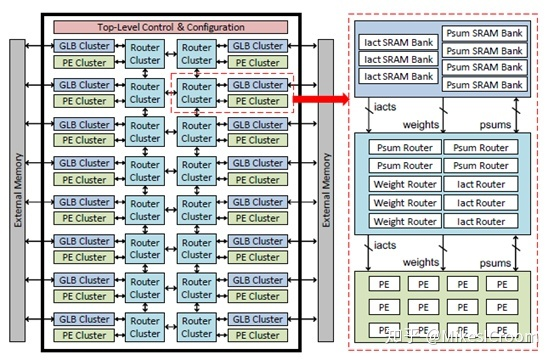
\includegraphics[width=7cm]{figure/eyerissv2.jpg} \\
    \caption{Architecture Diagram} 
   \label{fig.googles}
\end{figure}

\subsection{Design Description}

\subsection{High Level Timing Diagram}
\noindent\textit{\textcolor{blue}{Please provide the high level I/O timing diagram for the whole IP or SYS.}}

\subsection{Clock and Reset}
\noindent\textit{\textcolor{blue}{Please provide required clock and reset information in this chapter.}}

\subsubsection{Clock}
% Please add the following required packages to your document preamble:
% \usepackage[table,xcdraw]{xcolor}
% If you use beamer only pass "xcolor=table" option, i.e. \documentclass[xcolor=table]{beamer}
\begin{table}[hp]
    \centering
    \begin{tabularx}{\textwidth}{|X|X|X|X|X|}
    \hline
    \rowcolor[HTML]{009901} 
    {\color[HTML]{343434} \textbf{Clock Group}} & {\color[HTML]{343434} \textbf{Clock Name}} & {\color[HTML]{343434} \textbf{Frequency}} & {\color[HTML]{343434} \textbf{Duty Cycle}}     & {\color[HTML]{343434} \textbf{Accuracy}} \\ \hline
    {\color[HTML]{329A9D} \textbf{group 1}}     & {\color[HTML]{329A9D} \textbf{clk a}}      & {\color[HTML]{329A9D} \textbf{500MHz}}    & {\color[HTML]{329A9D} \textbf{45\%$\sim$55\%}} & {\color[HTML]{329A9D} \textbf{100ppm}}   \\ \hline
    {\color[HTML]{329A9D} \textbf{group 2}}     & {\color[HTML]{329A9D} \textbf{clk b}}      & {\color[HTML]{329A9D} \textbf{1GHz}}      & {\color[HTML]{329A9D} \textbf{45\%$\sim$55\%}} & {\color[HTML]{329A9D} \textbf{100ppm}}   \\ \hline
    {\color[HTML]{329A9D} \textbf{}}            & {\color[HTML]{329A9D} \textbf{}}           & {\color[HTML]{329A9D} \textbf{}}          & {\color[HTML]{329A9D} \textbf{}}               & {\color[HTML]{329A9D} \textbf{}}         \\ \hline
    \end{tabularx}
    \caption{Clock Requirements}
    \end{table}

\subsubsection{Reset}

\subsection{I/O Interfaces}

\noindent\textit{\textcolor{blue}{Please give the fully I/O interfaces in the interface table, the interfaces can be divided into different groups such as:}}
\begin{itemize}
    \item[\textcolor{blue}{$\bullet$}] \noindent\textit{\textcolor{blue}{Clock}}
    \item[\textcolor{blue}{$\bullet$}] \noindent\textit{\textcolor{blue}{Reset}}
    \item[\textcolor{blue}{$\bullet$}] \noindent\textit{\textcolor{blue}{Bus interfaces}}
\end{itemize}

\subsection{Interrupt}
\noindent\textit{\textcolor{blue}{Please list all interrupts detailed information in below table:}}

\subsection{Address Mapping}

